% 
% PROJECT PLAN DOCUMENT 
% =====================
% 
% Time-stamp: <2009-11-20 01:45:55 raskolnikov>
% (c) 2009 The JAGSAT development team.
% 

\documentclass[12pt,a4paper]{article}

\usepackage{raskolnikov}

\title{\large JAGSAT project\\\huge Project Plan Document}
\author{
  Juan Pedro Bolívar Puente\\ 
  Aksel Junkkila\\
  Guillem Medina\\ 
  Sarah Lindstrom\\ 
  Alberto Villegas Erce\\ 
  Thomas Forss
}
\location{Project Course \\ \textit{Åbo Akademy}}
% \date{}

\begin{document}
\maketitle

\tableofcontents
\pagebreak

\section{Project overview}

\subsection{Project objectives, goal}

Our project is to create a game for the gaming device that TribeFlame
is developing. The device will imitate board games, social and other
multi-player games through a computer with a multi-touch touch screen
as interface. Games will be downloadable through the TribeFlame online
store, which will work much like the mobile-phone stores (Appstore,
Ovi store). The games will be stored in the device which you can
easily carry with you wherever you go.

\subsection{Project deliverables}

The deliverables of this project will be:

\begin{itemize}
\item Project vision document
\item Project plan document
\item Project status reports and presentations
\item Design document
\item Business Documents and analysis (Venture Cup)
\item Poster
\item Postmortem analysis
\end{itemize}

\subsection{Budget and resources}

The project is done as a student project, no expenses. The team will
be using mainly computer resources available at Åbo Akademi.


\section{Project organization}

The project is lead by the project manager, Thomas Forss. The project
manager is responsible of planning and organization of the project,
and communication with customer. The project manager also is the team
leader for the team assigned to the project.

The team has additionally the following roles, as defined in table
\ref{tab:roles}.

\begin{table}[h!]
\small
\begin{tabular}{l|l}
Team member                                      &Role \\\hline\hline
Juan Pedro Bolívar Puente, Alberto Villegas Erce &Main programmers\\
Guillem Medina 					 &Programmer\\
Aksel Junkkila, Guillem Medina			 &Game designers\\		
Sarah Lindström, Thomas Forss			 &Business consultants\\
Alberto Villegas Erce, Aksel Junkkila		 &Documentation managers\\
Sarah Lindström					 &Usability manager\\
Juan Pedro Bolívar Puente			 &Unit test manager\\
\end{tabular}
\caption{Roles in the project.}
\label{tab:roles}
\end{table}

\section{Phases and milestones}

\subsection{Phases}
\begin{enumerate}
\item Specification phase
\item Design phase	
\item Implementation iterations:
\begin{enumerate}
\item Alpha version
\item Beta version
\item Quality assurance
\item Documentation
\item Bug fixes
\end{enumerate}
\end{enumerate}

\subsection{Milestones}

\begin{enumerate}
\item Specifications ready
	$\rightarrow$ 1.11.2009 (game defined)
\item Design version 1
	$\rightarrow$ 1.12.2009
\item Alpha release
	$\rightarrow$ 15.01.2009
\item Unofficial beta release
	$\rightarrow$ 12.02.2009 
\item Beta release
	$\rightarrow$ 12.03.2010
\item Passed quality assurance
	$\rightarrow$ 12.03.2009 (ICT  showroom)
\end{enumerate}

\subsection{Schedule}

\begin{figure}[h!]
\centering
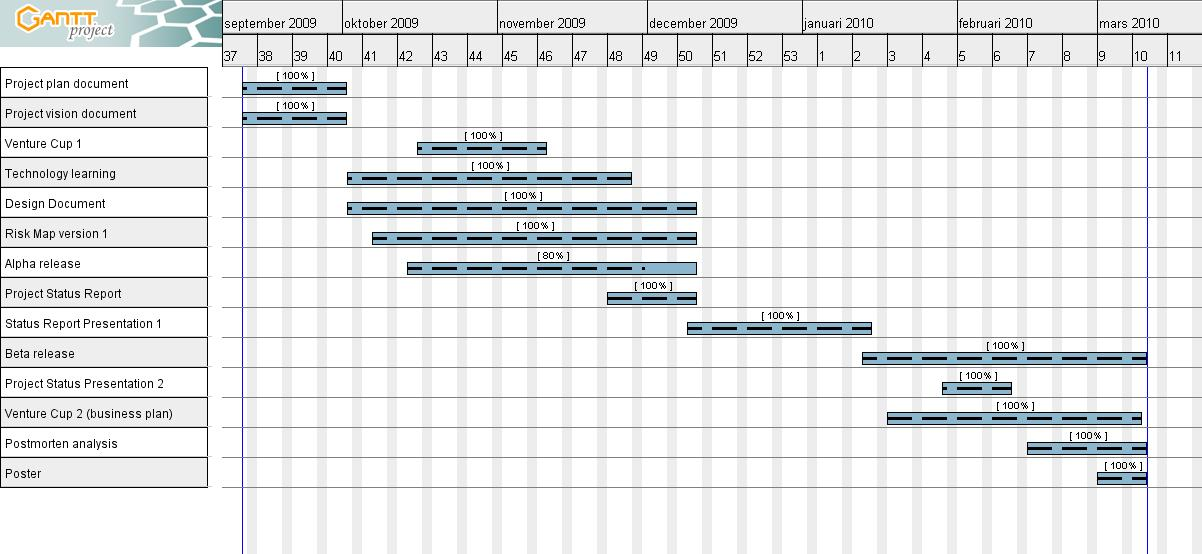
\includegraphics[width=13cm]{pic/gantt.jpg}
\caption{Gantt diagram.}
\label{fig:ganttdia}
\end{figure}

\subsection{Tasks}

The following tasks table has been defined as a guide for the project development. \ref{tab:tasks}

\begin{table}[h!]
\small
\begin{tabular}{ l | c | r | c}
Task				&Status		&Est. workload left (h)	&Deadline \\\hline\hline
Project Plan (2) 	&90	\%		&4					&14.12.2009\\
Project Vision (2)	&90 	\%		&4					&14.12.2009\\
Alpha release		&60 	\%		&220				&15.01.2010\\
\ - Core layer		&			&40					&\\
\ - In game menu	&			&20					&\\
\ - Main menu		&			&40					&\\
\ - Player menu		&			&10					&\\
\ - Map loading		&			&20					&\\
\ - Map component	&			&30					&\\
\ - Setup stage		&			&20					&\\
\ - Game stage		&			&20					&\\
\ - Integration		&			&20					&\\
Beta release		&10 \%		&100				&12.02.2010\\
\ - Load/Save game	&			&20					&\\
\ - Improving widgets	&			&30					&\\
\ - Art				&			&50					&\\
Venture Cup 2		&0 \%		&30					&11.03.2010\\
Beta release 2		&0 \%		&240				&12.03.2010\\
\ - Art				&			&40					&\\
\ - Programming	&			&200				&\\
Status report 2		&0 \%		&16					&12.03.2010\\
Risk Map ver. 2		&10 \%		&20					&12.03.2010\\
Graphics and sound	&0 \%		&12					&12.03.2010
\end{tabular}
\caption{Tasks}
\label{tab:tasks}
\end{table}


\section{Quality assurance}

The quality assurance will be performed inside the team. The
specifications are reviewed by the customer; the design is reviewed in
internal meetings.

Although we have a unit test manager in the group the code will always
be tested by one team member before forwarded. The whole group is
responsible for that the game works as planned and that quality
assurance phase is passed. We all have main responsibilities and
backups for each task.

\section{Risks}

In the project the following risks are identified:

\begin{itemize}
\item Availability of the resources. As the team members are working in the team besides other studies and activities, it is very difficult to guarantee the availability of the resources.
\item Dependency. This game depends on how the TribeFlame device works. Changes in the device may occur, and might make this project very sensitive.
\item Motivation. The team members are not motivated enough and may not finish the project on time.
\item Lack of knowledge. The programming language Python, which is new to a few team members, may prove to be more challenging than we thought in the beginning of the project.
\item Over ambitious. The team may plan a game which is not possible to program within the timeframe of the project.
\item Time table not estimated correctly. The schedule is not realistic and has to be revised during the project.
\item Injury, illness or other issues that prevent people from working. If this happens we will have to adjust the schedule and switch roles from back-up to main.
\end{itemize}

\section{Tracking}

\subsection{Project team meetings}

Meetings are held usually once a week. We will meet with Tribeflame
about once every two weeks. The meetings are recorded and conclusions
written down to be sent to everyone by e-mail.  We will keep track on
the work done with the JIRA task management system.

\subsection{Time tracking}

All time used for the project is recorded.  The time is recorded on ½
hour accuracy and categorized according to the following job types:
Meetings, programming, management, design, implementation, testing,
documentation, database, lectures.

\section{Documentation}

The system should mainly be self-explanatory, so user manual are not
really needed. However, the following basic documentation is needed:

\begin{description}
\item[Architectural manual] How the system is build up, which languages,
which basic data structures and mechanisms.  Installation manual: How
the system is installed in a new place.  Game manual: How to play the
game and how the game works in general.
\end{description}

\end{document}
